\documentclass[a4paper]{exam}

\usepackage{amsmath}
\usepackage{geometry}
\usepackage{graphicx}
\usepackage{hyperref}
\usepackage{pythonhighlight}

% \printanswers

\title{Weekly Challenge 01: Deterministic Finite Automata (DFA)}
\author{CS 212 Nature of Computation\\Habib University}
\date{Fall 2022}

\qformat{{\large\bf \thequestion. \thequestiontitle}\hfill}
\boxedpoints

\begin{document}
\maketitle

\begin{questions}

  \titledquestion{Acceptance by a DFA}

  A DFA is defined as a 5-tuple, $(Q, \Sigma, \delta, q_0, F)$. The computation it performs is to accept or reject a given string, $w$. We will program this computation.

  \paragraph{Tasks}
  \begin{itemize}
    \item In the accompanying file, \texttt{dfa.py}, implement the \textit{\_\_init\_\_} and \textit{accepts} methods. You may add other methods as needed. A description of the input to the \textit{\_\_init\_\_} method is given below.
  \end{itemize}

  \paragraph{Description} The list-of-strings representation of the DFA is as follows.
  \begin{itemize}
    \item The first string indicates the members of $Q$ as a space separated list.
    \item The next string indicates the members of $\Sigma$ as a space separated list.
    \item The next string indicates $q_0$.
    \item The next string indicates the members of $F$ as a space separated list.
    \item Each of the next $|Q|\times|\Sigma|$ strings indicates a different member of $\delta$ as a space separated list.
  \end{itemize}
  For example, below are the state diagram and string representations of a DFA.

  \begin{minipage}{0.6\linewidth}
    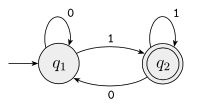
\includegraphics{example}
  \end{minipage}
  \begin{minipage}{0.2\linewidth}
    \begin{verbatim}
q1 q2
0 1
q1
q2
q1 0 q1
q1 1 q2
q2 0 q1
q2 1 q2
\end{verbatim}
  \end{minipage}

  \paragraph{Grading} Your score will be decided by the automated tests on GitHub. Please run \textit{pytest} locally before pushing to the repository. Course staff may call you for a viva, your performance on which may affect your score. Some sure-fire methods to score a 0 are:
  \begin{itemize}
    \item to hardcode for the provided testcases, and
    \item to submit plagiarized code.
  \end{itemize}

  \begin{solution}
    % Enter your solution here.
  \end{solution}
\end{questions}
\end{document}

%%% Local Variables:
%%% mode: latex
%%% TeX-master: t
%%% End:
